\documentclass{article}

\usepackage{mathrsfs,amsmath}
\usepackage{xcolor}
\usepackage{titlesec}
\usepackage{listings}
\usepackage{syntax}
\usepackage{pythonhighlighting}
\usepackage{graphicx}

\graphicspath{ {./assets/} }

\usepackage[margin=1.4in]{geometry}

\title{Handout \#9 | CS 471} 
\author{Jared Dyreson\\ 
        California State University, Fullerton}

\DeclareRobustCommand{\bowtie}{%
  \mathrel\triangleright\joinrel\mathrel\triangleleft}


\usepackage [english]{babel}
\usepackage [autostyle, english = american]{csquotes}
\MakeOuterQuote{"}

\titlespacing*{\section}
{0pt}{5.5ex plus 1ex minus .2ex}{4.3ex plus .2ex}
\titlespacing*{\subsection}
{0pt}{5.5ex plus 1ex minus .2ex}{4.3ex plus .2ex}

\usepackage{hyperref}
\hypersetup{
    colorlinks,
    citecolor=black,
    filecolor=black,
    linkcolor=black,
    urlcolor=black
}

\begin{document}

\maketitle
\tableofcontents

\newpage

\section{Questions}

\begin{enumerate}
\item What is the general structure of the HTTP response message?

\begin{figure}[!h]
\centering
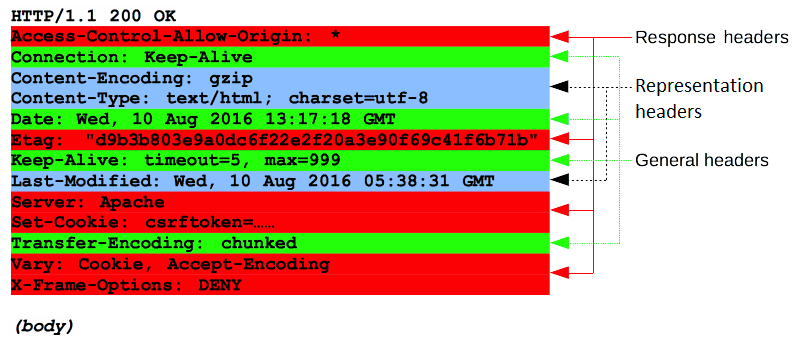
\includegraphics[width=10cm]{http_response_struct}
\end{figure}

\begin{itemize}
\item More information can be found \href{https://developer.mozilla.org/en-US/docs/Web/HTTP/Messages#http_responses}{\underline{here}}
\end{itemize}

\item What are the four basic components of a cookie system?

\begin{figure}[!h]
\centering
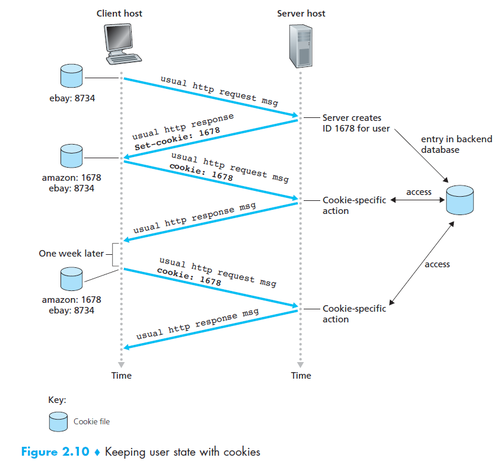
\includegraphics[width=7cm]{cookie_system}
\end{figure}

\begin{itemize}
\item A cookie header line in the HTTP response message
\item A cookie header line in the HTTP request message
\item A cookie file kept on the user's end system and managed by their browser
\item Back-end database at the website
\end{itemize}

\item Give an example of how web proxies can cheaply speed up internet access
\begin{itemize}
\item Cached data can be quickly dished out to the client and the server does not need to query the destination
\end{itemize}

\item Explain how the "If-modified-since" field is used
\begin{itemize}
\item It is used to dish out content only if the source material has been altered after a given date. This can be used in conjunction with a proxy server to speedup internet access and information retrieval.
\end{itemize}

\item FTP control connection is said to be "out-of-band". What does this mean?
\begin{itemize}
\item FTP uses two sockets; one for data transfer and the other to issue commands such as directory changes or file mode changes.
\item The use of the second socket constitutes it's name "out-of-band"
\end{itemize}

\item Compare HTTP and FTP
\begin{itemize}
\item HTTP is mainly used for static pages with simple text and images. FTP can support file transfers and interaction with the host file system.
\end{itemize}

\item Give a sequence of FTP commands for retrieving the file "file.txt" from the FTP server. You may assume any username and password.
\begin{verbatim}
USER username
PASSWORD password
RETR file.txt
\end{verbatim}

\item Is FTP stateful or stateless?
\begin{itemize}
\item The FTP connection will maintain state, as it needs to know which directory it is in, prior authentication, etc.
\end{itemize}
\end{enumerate}

\end{document}

